\documentclass[12pt]{article}
\usepackage[onehalfspacing]{setspace}
\usepackage{dcolumn}
\usepackage[left=1in, top=1in, bottom=1in]{geometry}
\usepackage{graphicx}
\usepackage[table,xcdraw]{xcolor}
\usepackage{longtable}
\usepackage{float}
\usepackage{listings}
\usepackage{xcolor}
\usepackage{amsmath}
\usepackage{amsfonts}
\usepackage{amssymb}


\lstset{language=R,
    basicstyle=\small\ttfamily,
    stringstyle=\color{commentgreen},
    otherkeywords={0,1,2,3,4,5,6,7,8,9},
    morekeywords={TRUE,FALSE},
    deletekeywords={data,frame,length,as,character},
    keywordstyle=\color{blue},
    commentstyle=\color{commentgreen},
}
\begin{document}

\title{Syndicate 5 Statistical Learning Problem Set \#2}
\maketitle
{\setlength{\parindent}{0cm}

\section*{Fishing Mode}
\subsection*{Ordered Logit Model}
An initial review of the data set identified that the price of beach and pier were identical. This was further highlighted in the correlation matrix in Appendix Table 1. The result confirmed that the beach price and pier price had a direct correlation of 1, as such, the beach price was not included in the model to avoid issues with multicollinearity. The boat and charter price and the boat and charter catch rate also had a strong correlation at 0.9963 and 0.9364, respectively. However, as the variables were not perfectly correlated, these predictors were retained in the model.\\

%% Correlation table to confirm multicollinearity
\begin{table}[!htbp] \centering 
  \caption{Correlation Matrix} 
  \label{} 
\resizebox{15cm}{!}{
\begin{tabular}{@{\extracolsep{5pt}} ccccccccc} 
\\[-1.8ex]\hline 
\hline \\[-1.8ex] 
 & price.beach & price.pier & price.boat & price.charter & catch.beach & catch.pier & catch.boat & catch.charter \\ 
\hline \\[-1.8ex] 
price.beach & $1$ & $1$ & $0.112$ & $0.141$ & $0.332$ & $0.226$ & $$-$0.098$ & $$-$0.027$ \\ 
price.pier & $1$ & $1$ & $0.112$ & $0.141$ & $0.332$ & $0.226$ & $$-$0.098$ & $$-$0.027$ \\ 
price.boat & $0.112$ & $0.112$ & $1$ & $0.996$ & $0.213$ & $0.253$ & $$-$0.041$ & $$-$0.023$ \\ 
price.charter & $0.141$ & $0.141$ & $0.996$ & $1$ & $0.245$ & $0.287$ & $$-$0.063$ & $$-$0.027$ \\ 
catch.beach & $0.332$ & $0.332$ & $0.213$ & $0.245$ & $1$ & $0.818$ & $0.139$ & $0.208$ \\ 
catch.pier & $0.226$ & $0.226$ & $0.253$ & $0.287$ & $0.818$ & $1$ & $0.134$ & $0.187$ \\ 
catch.boat & $$-$0.098$ & $$-$0.098$ & $$-$0.041$ & $$-$0.063$ & $0.139$ & $0.134$ & $1$ & $0.936$ \\ 
catch.charter & $$-$0.027$ & $$-$0.027$ & $$-$0.023$ & $$-$0.027$ & $0.208$ & $0.187$ & $0.936$ & $1$ \\ 
\hline \\[-1.8ex] 
\end{tabular} 
}
\end{table} 

An ordered logit model was then constructed to understand the relationship between a chosen mode of fishing and the price and catch rate for each mode, using the prescribed order of Beach $<$ Pier $<$ Boat $<$ Charter. The following results were obtained - refer to Appendix Table 2 for details.\\

$$y_i = \begin{cases}
1(Beach) & \text{if} \: z_i < 0.6893\\
2(Pier) & \text{if} \: 0.6893 leq z_i < 2.0414\\
3(Boat) & \text{if} \: 2.0414 \leq z_i < 3.9392\\
4(Charter) & \text{if} \: z_i \geq 3.9392
\end{cases}$$

$z_i = 0.0059Price.Pier_i - 0.1246Price.Boat_i + 0.1153Price.Charter_i + 0.6535Catch.Beach_i - 4.0614Catch.Pier_i + 0.9066Catch.Boat_i + 0.1986Catch.Charter_i + \varepsilon_i$\\

$\varepsilon_i \sim Logistic(\mu = 0, s = 1)$

%% Ordered Logit Model
\begin{table}[H] \centering 
  \caption{Ordered Logit Model} 
  \label{} 
\begin{tabular}{@{\extracolsep{5pt}}lc} 
\\[-1.8ex]\hline 
\hline \\[-1.8ex] 
 & \multicolumn{1}{c}{\textit{Dependent variable:}} \\ 
\cline{2-2} 
\\[-1.8ex] & mode \\ 
\hline \\[-1.8ex] 
 price.pier & 0.006$^{***}$ \\ 
  & (0.001) \\ 
  & \\ 
 price.boat & $-$0.125$^{***}$ \\ 
  & (0.014) \\ 
  & \\ 
 price.charter & 0.115$^{***}$ \\ 
  & (0.014) \\ 
  & \\ 
 catch.beach & 0.653 \\ 
  & (0.619) \\ 
  & \\ 
 catch.pier & $-$4.061$^{***}$ \\ 
  & (0.756) \\ 
  & \\ 
 catch.boat & 0.907 \\ 
  & (0.928) \\ 
  & \\ 
 catch.charter & 0.199 \\ 
  & (0.266) \\ 
  & \\ 
\hline \\[-1.8ex] 
Observations & 1,182 \\ 
\hline \\[-1.8ex] 
AIC & 2673.745 \\
\hline
\hline \\[-1.8ex] 
\textit{Note:}  & \multicolumn{1}{r}{$^{*}$p$<$0.1; $^{**}$p$<$0.05; $^{***}$p$<$0.01} \\ 
\end{tabular} 
\end{table} 

These results identified that the price of fishing at the pier/beach or on a charter increased the propensity for an individual to choose a charter. In contrast, the boat price decreased the propensity to choose a charter. All price predictors were statistically significant to a 0.001 level. These results were counterintuitive as an increase in charter price should intuitively reduce the propensity of a customer choosing a charter. This may point to a multicollinearity issue stemming from the strong correlation between boat and charter price. Examining the odds ratio plots in Appendix Figure 1, the first row of figures shows a general upward trend between each mode interval. This emphasised that as the price of fishing at the pier or beach increased, the odds of choosing a ‘higher’ mode of fishing increased at each interval. The opposite relationship is shown in the second row of plots where a general downward trend is illustrated, highlighting that the boat price is associated with a decrease in propensity to choose a charter at all mode intervals. Oddly, the charter price plots in the third row show a general downward trend which does not align with the sign of the estimated coefficient. Thus, further emphasizing potential multicollinearity.\\ 

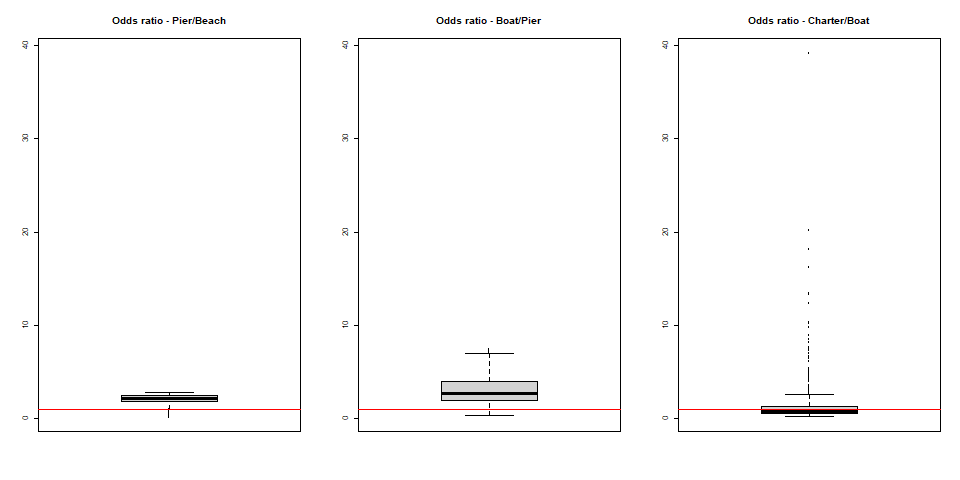
\includegraphics[scale=0.5]{Ordered Odds 1}\\

ooking at the catch rate, the pier catch rate was the only statistically significant predictor (to a significance level of 0.001). The pier catch rate had a negative relationship with the propensity to choose a charter i.e. as the catch rate at the pier increased, the likelihood of an individual choosing a charter decreased. Again, these results were unexpected as the boat or charter catch rate should intuitively have an influence on the mode choice. This may also point to a multicollinearity issue as the boat and charter catch rates were strongly correlated. Looking at the odds ratio plots shown in Appendix Figure 2 a clear trend with increasing pier catch rate is not shown. This may be an indicator that the catch rate does not explain as much of the variance in mode choice compared to price.\\

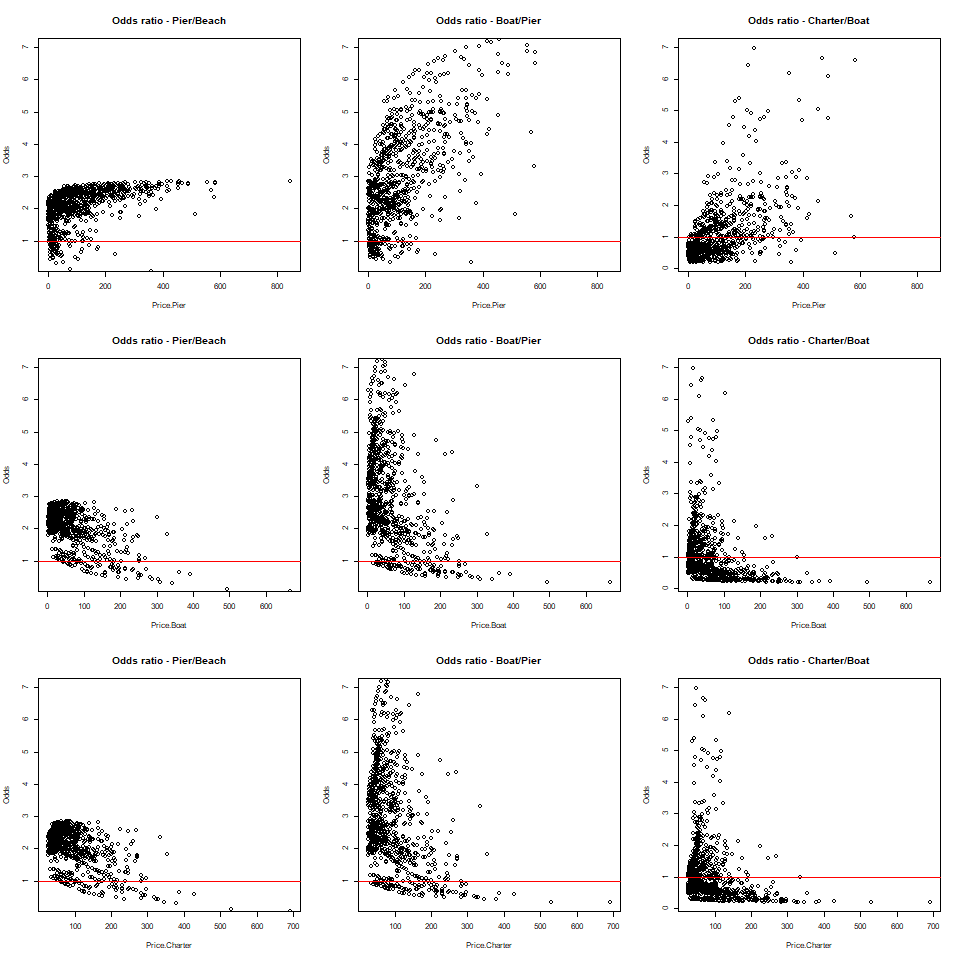
\includegraphics[scale=0.5]{Ordered Odds 2}\\
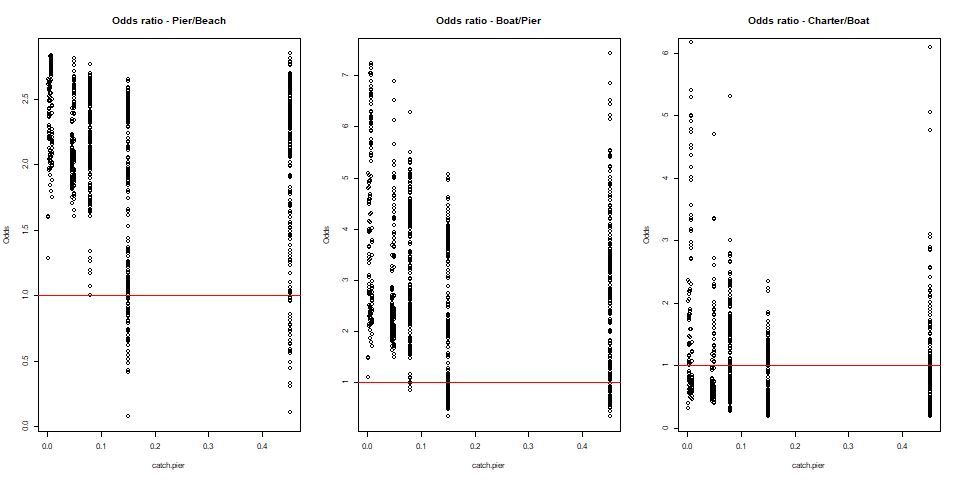
\includegraphics[scale=0.5]{Ordered Odds 3}\\


\subsection*{Multinomial Logit Model}
\subsubsection*{Question 1}

%% Multinomial Logit Model
\begin{table}[!htbp] \centering 
  \caption{Multinomial Logit Model} 
  \label{} 
\begin{tabular}{@{\extracolsep{5pt}} cccc} 
\\[-1.8ex]\hline 
\hline \\[-1.8ex] 
 & Boat & Charter & Pier \\ 
\hline \\[-1.8ex] 
(Intercept) & $$-$13.429^{***}$ & $$-$16.149^{***}$ & $$-$7.179^{**}$ \\ 
price.pier & $0.032^{***}$ & $0.027^{***}$ & $$-$0.005$ \\ 
price.boat & $$-$0.579^{***}$ & $$-$0.670^{***}$ & $$-$0.321^{***}$ \\ 
price.charter & $0.556^{***}$ & $0.652^{***}$ & $0.320^{***}$ \\ 
catch.beach & $58.579^{***}$ & $60.639^{***}$ & $37.511^{***}$ \\ 
catch.pier & $$-$86.664^{***}$ & $$-$86.885^{***}$ & $$-$51.327^{***}$ \\ 
catch.boat & $$-$0.521$ & $0.368$ & $$-$1.784$ \\ 
catch.charter & $0.306$ & $0.119$ & $0.100$ \\ 
\hline \\[-1.8ex] 
AIC & & 2181.346 \\
\hline
\hline \\[-1.8ex] 
\textit{Note:} & &  \multicolumn{1}{r}{$^{*}$p$<$0.1; $^{**}$p$<$0.05; $^{***}$p$<$0.01} \\ 
\end{tabular} 
\end{table} 

%% AIC
\begin{table}[!htbp] \centering 
  \caption{AIC for Multinomial Logit Model} 
  \label{} 
\begin{tabular}{@{\extracolsep{5pt}} c} 
\\[-1.8ex]\hline 
\hline \\[-1.8ex] 
$2,181.346$ \\ 
\hline \\[-1.8ex] 
\end{tabular} 
\end{table} 

\subsubsection*{Question 2}
The fundamental difference is that the choices in the ordered model have an order of agreed superiority while the multinomial model doesn't.\\

In our example, the ordered model assumes that everyone sees "Charter" as the best option, followed by "Boat", "Pier" and "Beach" respectfully. However, choices are influenced by the price and catch rates of each mode. Thus, the higher an individual's utility, the more likely they are to go with a "superior" option. Furthermore, in ordered models, there is no intercept as thresholds are estimated instead, making identification easier. Likelihoods are then allocated based on these thresholds and utilities.\\

For unordered outcomes, no preferences means that we must model probabilities relatively. Parameters are estimated for every group (except one reference group) to tell us the effect of a single change on each group and hence give the utility for each choice from which probabilities are allocated. Notably, there isn't an intercept estimated as thresholds aren't calculated.\\

For this fishing example, the unordered model is likely to be more suitable as individuals are unlikely to rank each mode the same due to personal preferences. This is backed up by the unordered model having a much lower AIC (2,181.346 vs 2673.745).









}
\end{document}